\documentclass[a4paper,twoside]{article}
\usepackage{geometry}
\geometry{margin=1cm,vmargin={0pt,1cm}}
\setlength{\topmargin}{-2cm}
\setlength{\paperheight}{23cm}
\setlength{\paperwidth}{18cm}
\setlength{\textheight}{19.6cm}
\setlength{\textwidth}{15cm}
\usepackage{makecell}
%\usepackage{fancyhdr}
\usepackage{siunitx}
\usepackage{amssymb}
\usepackage{indentfirst}
\setlength{\parindent}{0.5em}

\pagenumbering{arabic} 

% useful packages.
\usepackage{multirow}
\usepackage{caption}
\usepackage{mathrsfs}
\usepackage{amsfonts}
\usepackage{amsmath}
\usepackage{amsthm}
\usepackage{enumerate}
\usepackage{xcolor,graphicx,float,subfigure}
\usepackage{epstopdf}
\usepackage{multicol}
\usepackage{fancyhdr}
\usepackage{layout}
\usepackage{listings}
\usepackage{dsfont}
\lstset{language=Matlab}
\lstset{breaklines}
\lstset{extendedchars=false}
\usepackage[colorlinks,linkcolor=blue]{hyperref}
\usepackage{xcolor}
%\usepackage{cite}
%\usepackage[numbers,sort&compress]{natbib} 
%\setcitestyle{open={},close={}}
%\usepackage{natbibspacing}
%\renewcommand{\refname}{}
\usepackage{anyfontsize}

\usepackage{tikz}
\usetikzlibrary{calc}
\usetikzlibrary{arrows.meta}
\tikzset{
  dot/.style={
    circle, fill=black, inner sep=1pt, outer sep=0pt
  },
  dot label/.style={
    circle, inner sep=0pt, outer sep=1pt
  }
  arrow1/.style = {
    draw = black, thick, -{Latex[length = 4mm, width = 1.5mm]},
  }
}


% -------------------
% Theorem Environments
% -------------------
\theoremstyle{definition}
\newtheorem{thm}{Theorem}[section]
\newtheorem{prop}{Proposition}[section]
\newtheorem{lem}{Lemma}[section]
\newtheorem{coro}{Corollary}[section]

\newtheorem{exm}{Example}[section]
\newtheorem{nex}{Non-Example}[section]
\newtheorem{defn}{Definition}[section]
\theoremstyle{remark}
\newtheorem{rmk}{Remark}[section] 
\numberwithin{equation}{section}


\newcommand{\dif}{\mathrm{d}}
\newcommand{\avg}[1]{\left\langle #1 \right\rangle}
\newcommand{\difFrac}[2]{\frac{\dif #1}{\dif #2}}
\newcommand{\pdfFrac}[2]{\frac{\partial #1}{\partial #2}}
\newcommand{\OFL}{\mathrm{OFL}}
\newcommand{\UFL}{\mathrm{UFL}}
\newcommand{\fl}{\mathrm{fl}}
\newcommand{\op}{\odot}
\newcommand{\Eabs}{E_{\mathrm{abs}}}
\newcommand{\Erel}{E_{\mathrm{rel}}}

\newcommand{\Zero}{\hat{0}}
\newcommand{\One}{\hat{1}}
\newcommand{\Int}{\mathrm{int}}
\newcommand{\unitV}{\mathds{1}}

\newcommand{\bmi}{\mathbf{i}}
\newcommand{\bmj}{\mathbf{j}}
\newcommand{\bmn}{\mathbf{n}}

\newcommand{\dist}[2]{\text{dist}\left(#1, #2\right)}
\newcommand{\scientific}[2]{#1 \times 10^{#2}}


%\newcommand{\Dim}{{\mathbf{D}}}
\newcommand{\Dim}{{\scriptsize \textsf{D}}}
\newcommand{\me}{\mathrm{e}}
\newcommand{\mi}{\mathrm{i}}

%\newcommand{\mod}{\mathrm{mod}}
\newcommand{\curve}[1]{\widetilde{#1}}
%\newcommand{\dt}{\delta t}
\newcommand{\dt}{\tau}
\newcommand{\isCovered}{\mathbin{ < \! \! \! \! \cdot }}
%\newcommand{\cIncluded}{\mathbin{ \prec \! \! \! \cdot }}
\newcommand{\coveredBy}{\lhd}
%\newcommand{\regrz}[1]{\mathrm{cl}\left(\mathrm{int}\left(#1\right)\right)}
\newcommand{\regrz}[1]{\mathrm{reg}\left(#1\right)}
%\newcommand{\sgncup}{\ \hat{\cup} \ }
\newcommand{\Span}{\mathrm{span}}
\newcommand{\timeline}[2]{\phi_{t_0}^{#1}\left( #2 \right)}
\newcommand{\timeBP}[1]{\overleftarrow{#1}}
\newcommand{\timeBPA}[1]{\mathring{\overleftarrow{#1}}}
\newcommand{\streak}[2]{\Psi_{t_0}^{#1}\left(#2\right)}
\newcommand{\timelineA}[2]{\mathring{\phi}_{t_0,#2}^{#1}}
\newcommand{\DRLN}[1]{{\cal D}_{\curve{#1}}}
\newcommand{\DRLLN}[1]{{\cal D}_{\overline{#1}}}
\newcommand{\DRLNA}[1]{\mathring{\cal D}_{\curve{#1}}}
%\newcommand{\oplusDR}{\,\overline{\oplus}\,}
\newcommand{\oplusDR}{\,\bar{\oplus}\,}
\newcommand{\qo}{\hat{q}}
\newcommand{\xo}{\hat{x}}
\newcommand{\yo}{\hat{y}}
\newcommand{\closure}[1]{\textrm{cl}\left(#1\right)}
\newcommand{\vertexSequence}[4]{
  \left( #1 \rightarrow #2 \rightarrow #3 \rightarrow #4 \rightarrow #1\right)}

\newcommand{\ppSpace}{\Pi_{<\kappa,\bm{\xi},\bm{\nu}}}
\newcommand{\pnSpace}{\mathbb{P}_{<\kappa}}
\newcommand{\pnSpaceK}[1]{\mathbb{P}_{#1}}

\newcommand{\Pyr}[2]{\textrm{Pyr}_{\cal{#1}}\left(\mathbf{#2}\right)}

%\pagestyle{plain}
\pagestyle{fancy}
\fancyhf{}
\fancyhead[LE,RO]{\textbf{\thepage}}

\makeatletter
\newcommand\sixteen{\@setfontsize\sixteen{17pt}{6}}
\renewcommand{\maketitle}{\bgroup\setlength{\parindent}{0pt}
\begin{flushleft}
\sixteen\bfseries \@title
\medskip
\end{flushleft}
\textit{\@author}
\egroup}
\makeatother


\title{Modern C++ Design}


\begin{document}
\maketitle

\section{Policy-Based Class Design}

In brief, policy-based class design
fosters assembling a class with complex behavior out of many little classes 
(called policies), each of which
takes care of only one behavioral or structural aspect.

The generic SingletonHolder class \textbf{template} (Chapter
6) uses policies for managing lifetime and thread safety. {SmartPtr} (Chapter 7) 
is built almost entirely from policies. The \textbf{double-dispatch engine} in Chapter 11 
uses policies for selecting various trade-offs. The
generic \textbf{Abstract Factory} implementation in Chapter 9 uses a policy for choosing a
creation method.

\subsection{Failure of the Do-it-all Interface}

Implementing everything under the umbrella of a do-it-all interface is not a good solution, for several
reasons:

\begin{itemize}
    \item Intellectual overhead, sheer size, and inefficiency.
    \item Loss of static type safety. A design should enforce most constraints at compile time. (No two singleton objects)
\end{itemize}

\subsection{Multiple Inheritance to the Rescue?}
For example, the user would build a multi-threaded, reference-counted smart pointer
class by inheriting some 
\texttt{BaseSmartPtr} class and two classes: \texttt{MultiThreaded}
and  \texttt{RefCounted}. Any experienced class 
designer knows that such a naive design does not work.

The problems with assembling separate features by using
multiple inheritance are as follows:
\begin{itemize}
\item \textbf{Mechanics}. There is no boilerplate code to assemble the
  inherited components in a controlled manner. \textbf{The language applies
  simple superposition in combining the base classes and establishes a
  set of simple rules for accessing their members.  }
\item \textbf{Type information}. The base classes do not have enough type
  information to carry out their tasks. 
\item \textbf{State manipulation}. Various behavioral aspects implemented with
  base classes must manipulate the same state. This means that they
  must use virtual inheritance to inherit a base class that holds the
  state. This complicates the design and makes it more rigid because
  the premise was that user classes inherit library classes, not vice versa.
\end{itemize}

\subsection{Templates}

Benefits:
\begin{itemize}
\item Class templates are customizable in ways not supported by
  regular classes.
\item for class templates with multiple parameters, you can use
  partial template specialization.
\end{itemize}

As soon as you try to implement such designs, you stumble upon several
problems that are not self-evident:
\begin{itemize}
\item You cannot specialize structure.
\item Specialization of member functions does not scale: you cannot
  specialize individual member functions for templates with multiple
  template parameters.
\item The library writer cannot provide multiple \textbf{default} values.
\end{itemize}

Multiple inheritance and templates foster complementary trade-offs:
\begin{itemize}
\item Multiple inheritance has scarce mechanics; templates have rich
mechanics
\item Multiple inheritance loses type information, which abounds
in templates.
\item Specialization of templates does not scale, but multiple
inheritance scales quite nicely.
\item You can provide only one default for
a template member function, but you can write an unbounded 
number of base classes.
\end{itemize}

\subsection{Policy Classes}

A \textbf{policy} defines a class interface or a class template interface. The
interface consists of one or all of the following: \textbf{inner type
definitions, member functions, and member variables}. The
implementations of a policy are called \textbf{policy classes}. Policy classes
are not intended for stand-alone use; instead, they are inherited by,
or contained within, other classes.

\begin{verbatim}
template <class T>
struct OpNewCreator{
  static T* Create(){
    return new T;
  }
};

template <class T>
struct MallocCreator{
  static T* Create(){
    void* buf = std::malloc(sizeof(T));
    if (!buf) return 0;
    return new(buf) T;
  }
};

template <class T>
struct PrototypeCreator{
  PrototypeCreator(T* pObj = 0):pPrototype_(pObj){}
  T* Create(){
    return pPrototype_ ? pPrototype_->Clone() : 0;
  }
  T* GetPrototype() { return pPrototype_; }
  void SetPrototype(T* pObj) { pPrototype_ = pObj; }
private:
  T* pPrototype_;
};
\end{verbatim}

The classes that use one or more policies are called hosts or
\textbf{host classes}.

\begin{verbatim}
template <class CreationPolicy>
class WidgetManager : public CreationPolicy{
  ...
};
typedef WidgetManager< OpNewCreator<Widget> > MyWidgetMgr;
\end{verbatim}

\textbf{It is the user of \texttt{WidgetManager} who chooses the creation
  policy}. This is the gist of policy-based class design.

\subsection{Implementing Policy Classes with Template Template
  Parameters}

The policy's template argument is redundant. In this case, we can use
\textbf{template template parameters} for specifying policies, as shown in the
following:
\begin{verbatim}
template <template <class> class CreationPolicy = OpNewcreator>
class WidgetManager : public CreationPolicy<Widget>{
  ...
};
typedef WidgetManager<OpNewCreator> MyWidgetMgr;
\end{verbatim}

Using template template parameters with policy classes is not simply a
matter of convenience; sometimes, it is essential that the host class
have access to the template so that the host can instantiate it with a
different type. For example:

\begin{verbatim}
template <template <class> class CreationPolicy = OpNewcreator>
class WidgetManager : public CreationPolicy<Widget>{
  void DoSomething(){
    Gadget* pW = CreationPolicy<Gadget>().Create();
  }
};
\end{verbatim}

Benefits of using policies:
\begin{itemize}
\item you can change policies from theoutside as easily as changing a
  template argument when you instantiate \texttt{WidgetManager}.
\item you can provide your own policies that are specific to your
  concrete application.
\item Policies allow you to generate designs by combining simple
  choices in a typesafe manner.
\item the binding between a host class and its policies is done at
  compile time, the code is tight and efficient, comparable to its
  handcrafted equivalent.
\end{itemize}

\subsection{Destructors of Policy Classes}

The user can automatically convert a host class to a policy and later
\texttt{delete} that pointer. Unless the policy class defines a virtual
destructor, applying delete to a pointer to the policy class has
undefined behavior.

Defining a virtual destructor for a policy, however, works against its
static nature and hurts performance. The lightweight, effective
solution that policies should use is to define a nonvirtual protected
destructor:
\begin{verbatim}
template <class T>
struct OpNewCreator{
protected:
  ~OpNewCreator() {}
};
\end{verbatim}

Because the destructor is protected, \textbf{only derived classes can destroy
policy objects}, so it's impossible for outsiders to apply delete to a
pointer to a policy class.

\subsection{Enriched Policies}

The \texttt{Creator} policy prescribes only one member function,
\texttt{Create}. However, \texttt{PrototypeCreator} defines two more functions:
\texttt{GetPrototype} and \texttt{SetPrototype}.

A user who uses a prototype-based Creator policy class can write the
following code: 
\begin{verbatim}
typedef WidgetManager<PrototypeCreator> MyWidgetManager;

Widget* pPrototype = ...;
MyWidgetManager mgr;
mgr.SetPrototype(pPrototype);
\end{verbatim}

If the user later decides to use a creation policy that does not
support prototypes, \textbf{the compiler pinpoints the spots where the
prototype-specific interface was used.} This is exactly what should be
expected from a sound design.

\subsection{Optional Functionality Through Incomplete Instantiation}

If a member function of a class template is never used, \textbf{it is not even
instantiated—the compiler does not look at it at all}, except perhaps
for syntax checking.

\begin{verbatim}
template <template <class> class CreationPolicy>
class WidgetManager : public CreationPolicy<Widget>{
  void SwitchPrototype(Widget* pNewPrototype){
    CreationPolicy<Widget>& myPolicy = *this;
    delete myPolicy.GetPrototype();
    myPolicy.SetPrototype(pNewPrototype);
  }
};
\end{verbatim}
The resulting context is very interesting:
\begin{itemize}
\item If the user instantiates \texttt{WidgetManager} with a Creator
  policy class that does not support prototypes and tries to use
  \texttt{SwitchPrototype}, a compile-time error occurs.
\item  If the user instantiates \texttt{WidgetManager} with a Creator
  policy class that does not support prototypes and does not try to
  use \texttt{SwitchPrototype}, the program is valid.
\end{itemize}
This all means that \texttt{WidgetManager} can benefit from optional
enriched interfaces but still work correctly with poorer interfaces.

\subsection{Compatible and Incompatible Policies}

Suppose you create two instantiations of \texttt{SmartPtr }:
\texttt{FastWidgetPtr}, a pointer with out checking, and 
\texttt{SafeWidgetPtr}, a pointer with checking before dereference.
It is natural to accept the conversion from \texttt{FastWidgetPtr} to
\texttt{SafeWidgetPtr}, but freely converting \texttt{SafeWidgetPtr}
objects to \texttt{FastWidgetPtr} objects is dangerous. 

The best, most scalable way to implement conversions between policies
is to initialize and copy \texttt{SmartPtr} objects policy by policy,
as shown below:

\begin{verbatim}
template<class T,template <class> class CheckingPolicy>
class SmartPtr : public CheckingPolicy<T>{
  template<class T1,template <class> class CP1,>
  SmartPtr(const SmartPtr<T1, CP1>& other)
    : pointee_(other.pointee_), CheckingPolicy<T>(other){ ... }
};
\end{verbatim}

When you initialize a \texttt{SmartPtr<Widget, EnforceNotNull> } with a
\texttt{SmartPtr<ExtendedWidget, NoChecking>}. The compiler tries to
match \texttt{SmartPtr<ExtendedWidget, NoChecking>} to
\texttt{EnforceNotNull}'s constructors.

If \texttt{EnforceNotNull}
implements a \textbf{constructor} that accepts a \texttt{NoChecking} object,
then the compiler matches that constructor. If \texttt{NoChecking}
implements a \textbf{conversion} operator to \texttt{EnforceNotNull}, that 
conversion is invoked. In any other case, the code fails to compile.

Although conversions from \texttt{NoChecking} to
\texttt{EnforceNotNull} and even vice versa are quite sensible, some
conversions don't make any sense at all.  As soon as you try to
confine a pointer to another ownership policy, you break the invariant
that makes reference counting work.

In conclusion, conversions that change the ownership policy should not
be allowed implicitly and should be treated with maximum care.

\subsection{ Decomposing a Class into Policies}

Two policies that do not interact with each other are orthogonal. By
this definition, the Array and the Destroy policies are not
orthogonal.

Nonorthogonal policies are an imperfection you should strive to
avoid. \textbf{They reduce compile-time type safety and complicate the design
  of both the host class and the policy classes.}

If you must use nonorthogonal policies, you can minimize dependencies
by passing a policy class as an argument to another policy class's
template function. However, this decreases encapsulation.
%%% Local Variables:
%%% mode: latex
%%% TeX-master: "../DesignPattern.tex"
%%% End:


\newpage
\section{Techniques}

\subsection{Compile-Time Assertions}

\textbf{C++17 provides \texttt{static\_assert}}.

The simplest solution to compile-time assertions works in C as well as in
C++, relies on the fact that a zero-length array is illegal.

\begin{verbatim}
#define STATIC_CHECK(expr) { char unnamed[(expr) ? 1 : 0]; }
template <class To, class From>
To safe_reinterpret_cast(From from){
  STATIC_CHECK(sizeof(From) <= sizeof(To));
  return reinterpret_cast<To>(from);
}
void* somePointer = ...;
char c = safe_reinterpret_cast<char>(somePointer);
\end{verbatim}

The problem with this approach is that the error message you receive
is not terribly informative. Error messages have no rules that they
must obey; it's all up to the compiler.

A better solution is to rely on a template with an informative name;
with luck, the compiler will mention the name of that template in the
error message.

\begin{verbatim}
template<bool> struct CompileTimeError;
template<> struct CompileTimeError<true> {};
#define STATIC_CHECK(expr) \
(CompileTimeError<(expr) != 0>())
\end{verbatim}

If you try to instantiate
\texttt{CompileTimeError<false>}, the compiler utters a message such
as "Undefined specialization \texttt{CompileTimeError<false>}." This
message is a slightly better hint that the error is intentional and
not a compiler or a program bug.

Actually, the name \texttt{CompileTimeError} is no longer suggestive
in the new context. \textbf{The ellipsis means the constructor accepts anything.}

\begin{verbatim}
template<bool> struct CompileTimeChecker{
  CompileTimeChecker(...);
};
template<> struct CompileTimeChecker<false> { };
#define STATIC_CHECK(expr, msg) {\
  class ERROR_##msg {}; \
  (void)sizeof(CompileTimeChecker<(expr) != 0>((ERROR_##msg())));\
}

template <class To, class From>
To safe_reinterpret_cast(From from){
  STATIC_CHECK(sizeof(From) <= sizeof(To),Destination_Type_Too_Narrow);
  return reinterpret_cast<To>(from);
}
void* somePointer = ...;
char c = safe_reinterpret_cast<char>(somePointer);
\end{verbatim}

After macro preprocessing, the code of \texttt{safe\_reinterpret\_cast}
expands to the following:

\begin{verbatim}
template <class To, class From>
To safe_reinterpret_cast(From from){
  class ERROR_Destination_Type_Too_Narrow {};
  (void)sizeof(
    CompileTimeChecker<(sizeof(From) <= sizeof(To))>(
      ERROR_Destination_Type_Too_Narrow()));
  return reinterpret_cast<To>(from);
}
\end{verbatim}

The \texttt{CompileTimeChecker<true>} specialization has a constructor
that accept anything; it's an ellipsis function. If the comparison
between sizes evaluates to false, a decent compiler outputs an error
message such as "Error: Cannot convert
\texttt{ERROR\_Destination\_Type\_Too\_Narrow} to
\texttt{CompileTimeChecker <false>}.

\subsection{Partial Template Specialization}

\begin{verbatim}
template <class Window, class Controller>
class Widget{
  ... generic implementation ...
};

// Partial specialization of Widget
template <class Window>
class Widget<Window, MyController>{
  ... partially specialized implementation ...
};

template <class ButtonArg>
class Widget<Button<ButtonArg>, MyController>{
  ... further specialized implementation ...
};
\end{verbatim}

Unfortunately, partial template specialization does not apply to
functions—be they member or nonmember—which somewhat reduces the
flexibility and the granularity of what you can do:
\begin{itemize}
\item Although you can \textbf{totally specialize} member functions of
  a class template, you cannot \textbf{partially specialize} member
  functions.
\item You cannot partially specialize namespace-level (nonmember)
  template functions. The closest thing to partial specialization for
  namespace-level template functions is overloading (not for changing the
  return value or for internally used type).
\end{itemize}

\begin{verbatim}
template <class T, class U> T Fun(U obj); // primary template
template <class U> void Fun<void, U>(U obj); // illegal partial specialization
template <class T> T Fun (Window obj); // legal (overloading)
\end{verbatim}

\subsection{Local Classes}

\textbf{Local classes cannot define static member variables and cannot
  access nonstatic local variables}. What makes local classes truly
interesting is that you can use them in template functions. \textbf{Local
classes defined inside template functions can use the template
parameters of the enclosing function.}

\begin{verbatim}
class Interface{
public:
virtual void Fun() = 0;
};
template <class T, class P>
Interface* MakeAdapter(const T& obj, const P& arg){
  class Local : public Interface{
  public:
    Local(const T& obj, const P& arg): obj_(obj), arg_(arg) {}
    virtual void Fun(){
      obj_.Call(arg_);
    }
  private:
     T obj_;
     P arg_;
  };
  return new Local(obj, arg);
}
\end{verbatim}

It can be easily proven that any idiom that uses a local class can be
implemented using a template class outside the function. On the other
hand, local classes can simplify implementations and improve locality
of symbols.

Local classes do have a unique feature, though: They are
\textbf{final}. Outside users cannot derive from a class hidden in a
function. Without local classes, you'd have to add an unnamed
namespace in a separate translation unit.

\subsection{Mapping Integral Constants to Types}

\begin{verbatim}
template <int v>
struct Int2Type{
enum { value = v };
};
\end{verbatim}

\texttt{Int2Type} generates a distinct type for each distinct constant
integral value passed.  You can use \texttt{Int2Type} whenever you
need to "typify" an integral constant quickly. This way you can 
\textbf{select different functions, depending on the result of a
  compile-time calculation.} Effectively, you \textbf{achieve static
  dispatching on a constant integral value. }

For dispatching at runtime, you can use simple \texttt{if-else}
statements or the \texttt{switch} statement.  However, the
\texttt{if-else} statement requires both branches to compile
successfully, even when the condition tested by \texttt{if} is known
at compile time.

\begin{verbatim}
template <typename T, bool isPolymorphic>
class NiftyContainer{
  void DoSomething(){
    T* pSomeObj = ...;
    if (isPolymorphic){
      T* pNewObj = pSomeObj->Clone();
      ... polymorphic algorithm ...
    }
    else{
      T* pNewObj = new T(*pSomeObj);
      ... nonpolymorphic algorithm ...
    }
  }
};
\end{verbatim}

The polymorphic algorithm uses \texttt{pObj->Clone()},
\texttt{NiftyContainer::DoSomething }does not compile for any type
that doesn't define a member function \texttt{Clone()}.

If \texttt{T} has disabled its copy constructor (by making it
private), if \texttt{T} is a polymorphic type and the nonpolymorphic
code branch attempts \texttt{new T(*pObj)}, the code might fail to
compile.

\begin{verbatim}
template <typename T, bool isPolymorphic>
class NiftyContainer{
private:
  void DoSomething(T* pObj, Int2Type<true>){
    T* pNewObj = pObj->Clone();
    ... polymorphic algorithm ...
  }
  void DoSomething(T* pObj, Int2Type<false>){
    T* pNewObj = new T(*pObj);
    ... nonpolymorphic algorithm ...
  }
public:
  void DoSomething(T* pObj){
    DoSomething(pObj, Int2Type<isPolymorphic>());
  }
};
\end{verbatim}

\textbf{There is another solution, \texttt{if constexpr()}, the new
  feature provided by c++17.}

\subsection{Type-to-Type Mapping}

\begin{verbatim}
template <class T, class U>
T* Create(const U& arg){
  return new T(arg);
}
\end{verbatim}

If objects of type \texttt{Widget} are untouchable legacy code and must
take two arguments upon construction, the second being a fixed value
such as -1. How can you specialize Create so that it treats \texttt{Widget}
differently from all other types with a uniform interface?

\begin{verbatim}
// Illegal code — don't try this at home
template <class U>
Widget* Create<Widget, U>(const U& arg){
  return new Widget(arg, -1);
}

// rely on overloading
template <class T, class U>
T* Create(const U& arg, T /* dummy */){
  return new T(arg);
}
template <class U>
Widget* Create(const U& arg, Widget /* dummy */){
  return new Widget(arg, -1);
}
\end{verbatim}

Such a solution would incur the overhead of constructing an
arbitrarily complex object that remains unused.

\begin{verbatim}
template <typename T>
struct Type2Type{
  typedef T OriginalType;
};
template <class T, class U>
T* Create(const U& arg, Type2Type<T>){
  return new T(arg);
}
template <class U>
Widget* Create(const U& arg, Type2Type<Widget>){
  return new Widget(arg, -1);
}
// Use Create()
String* pStr = Create("Hello", Type2Type<String>());
Widget* pW = Create(100, Type2Type<Widget>());
\end{verbatim}

\subsection{Type Selection}

Sometimes generic code needs to select one type or another, depending
on a Boolean constant.

You might want to use an \texttt{std::vector} as your back-end
storage. Obviously, you cannot store polymorphic types by value, so
you must store pointers. On the other hand, you might want to store
nonpolymorphic types by value, because this is more efficient.

\begin{verbatim}
template <typename T, bool isPolymorphic>
struct NiftyContainerValueTraits{
  typedef T* ValueType;
};
template <typename T>
struct NiftyContainerValueTraits<T, false>{
  typedef T ValueType;
};
template <typename T, bool isPolymorphic>
class NiftyContainer{
  typedef NiftyContainerValueTraits<T, isPolymorphic> Traits;
  typedef typename Traits::ValueType ValueType;
};
\end{verbatim}

This way of doing things is unnecessarily clumsy. Moreover, it doesn't
scale: For each type selection, you must define a new traits class
template.

\begin{verbatim}
template <bool flag, typename T, typename U>
struct Select{
  typedef T Result;
};
template <typename T, typename U>
struct Select<false, T, U>{
  typedef U Result;
};

template <typename T, bool isPolymorphic>
class NiftyContainer{
  typedef typename Select<isPolymorphic, T*, T>::Result ValueType;
}
\end{verbatim}

\subsection{Detecting Convertibility and Inheritance at Compile Time}

 In a generic function, you can rely on an optimized algorithm if a
 class implements a certain interface. Discovering this at compile
 time means not having to use \texttt{dynamic\_cast}, which is costly
 at runtime.

 Detecting inheritance relies on a more general mechanism, that of
 detecting convertibility. The more general problem is, How can you
 detect whether an arbitrary type \texttt{T} supports automatic
 conversion to an arbitrary type \texttt{U}?

 There is a surprising amount of power in \texttt{sizeof}: You can
 apply \texttt{sizeof} to any expression, no matter how complex, and
 \texttt{sizeof} \textbf{returns its size without actually evaluating
   that expression at runtime. }

 The idea of conversion detection relies on using \texttt{sizeof} in
 conjunction with overloaded functions. We provide two overloads of a
 function: \textbf{One accepts the type to convert to (\texttt{U}), and the
 other accepts just about anything else. } If the function that
accepts a \texttt{U} gets called, we know that \texttt{T} is
convertible to \texttt{U}.

\begin{verbatim}
typedef char Small;
class Big { char dummy[2]; };
Small Test(U);
Big Test(...);
const bool convExists = sizeof(Test(T())) == sizeof(Small);
\end{verbatim}
Passing a C++ object to a function with ellipses has undefined
results, but this doesn't matter. Nothing actually calls the
function. It's not even implemented. Recall that \texttt{sizeof} does
not evaluate its argument.

There is one little problem. If \texttt{T} makes its default constructor
private, the expression \texttt{T()} fails to compile. Fortunately,
there is a simple solution, just use a strawman function
returning a \texttt{T}.  \texttt{MakeT} and \texttt{Test} not only
don't do anything but don't even really exist at all.

\begin{verbatim}
template <class T, class U>
class Conversion{
  typedef char Small;
  class Big { char dummy[2]; };
  static Small Test(U);
  static Big Test(...);
  static T MakeT(); // not implemented
public:
  enum { exists = sizeof(Test(MakeT())) == sizeof(Small) };
};
cout << Conversion<size_t, vector<int> >::exists << ' ';
// return 0, because that constructor is explicit.
\end{verbatim}

We can implement one more constant inside
\texttt{Conversion::sameType}, which is true if \texttt{T} and
\texttt{U} represent the same type:

\begin{verbatim}
template <class T, class U>
class Conversion{
  ... as above ...
  enum { sameType = false };
};
template <class T>
class Conversion<T, T>{
public:
  enum { exists = 1, sameType = 1 };
};
#define SUPERSUBCLASS(T, U) \
(Conversion<const U*, const T*>::exists && \
!Conversion<const T*, const void*>::sameType)
\end{verbatim}

There are only three cases in which \texttt{const U*} converts
implicitly to \texttt{const T*}: 
\begin{enumerate}
\item \texttt{T} is the same type as \texttt{U}
\item \texttt{T} is an unambiguous public base of \texttt{U}
\item \texttt{T} is \texttt{void}.
\end{enumerate}

Using \texttt{const} in \texttt{SUPERSUBCLASS}, we're always on the
safe side, we don't want the conversion test to fail due to
\texttt{const} issues.

Why use \texttt{SUPERSUBCLASS} and not the cuter \texttt{BASE\_OF} or
\texttt{INHERITS}? Think with \texttt{INHERITS(T, U)} it was a
constant struggle to say which way the test worked.

\subsection{A Wrapper Around \texttt{type\_info} }

tandard C++ provides the \texttt{std::type\_info} class, which gives you the
ability to investigate object types at runtime. You typically use
\texttt{type\_info} in conjunction with the \texttt{typeid}
operator. The \texttt{typeid} operator returns a reference to a
\texttt{type\_info} object:

\begin{verbatim}
void Fun(Base* pObj){
  // Compare the two type_info objects corresponding to the type of *pObj and Derived
  if (typeid(*pObj) == typeid(Derived)){
    ... aha, pObj actually points to a Derived object ...
  }
}
\end{verbatim}

In addition to supporting the comparison operators \texttt{operator==}
and \texttt{operator!=}, \texttt{type\_info} provides two more
functions:

\begin{enumerate}
\item The \texttt{name} member function returns a textual
  representation of a type, in the form of \texttt{const char*}.
\item he before member function introduces an implementation's
  collation ordering relationship for \texttt{type\_info} objects.
\item The \texttt{type\_info} class disables the copy constructor and
  assignment operator, which makes storing \texttt{type\_info} objects
  impossible.
\item The objects returned by \texttt{typeid} have static storage, so
  you don't have to worry about lifetime issues.  
\end{enumerate}

You do have to worry about pointer identity, the standard does not
guarantee that each invocation returns a reference to the same
\texttt{type\_info} object. Consequently, you cannot compare pointers
to \texttt{type\_info} objects. What you should do is to store pointers
to \texttt{type\_info} objects and compare them by applying
\texttt{type\_info::operator==} to the dereferenced pointers.

If you want to use STL's ordered containers with \texttt{type\_info},
you must write a little functor and deal with pointers. All this is
clumsy enough to mandate a wrapper class around \texttt{type\_info}
that stores a pointer to a \texttt{type\_info} object and provides:
\begin{enumerate}
\item All member functions of \texttt{type\_info}
\item Value semantics (public copy constructor and assignment
  operator)
\item Seamless comparisons by defining \texttt{operator<} and
  \texttt{operator==}
\end{enumerate}

\begin{verbatim}
class TypeInfo{
public:
  // Constructors/destructors
  TypeInfo(); // needed for containers
  TypeInfo(const std::type_info&);
  TypeInfo(const TypeInfo&);
  TypeInfo& operator=(const TypeInfo&);
  // Compatibility functions
  bool before(const TypeInfo&) const;
  const char* name() const;
private:
  const std::type_info* pInfo_;
};
// Comparison operators
bool operator==(const TypeInfo&, const TypeInfo&);
bool operator!=(const TypeInfo&, const TypeInfo&);
bool operator<(const TypeInfo&, const TypeInfo&);
bool operator<=(const TypeInfo&, const TypeInfo&);
bool operator>(const TypeInfo&, const TypeInfo&);
bool operator>=(const TypeInfo&, const TypeInfo&);

void Fun(Base* pObj){
  TypeInfo info = typeid(Derived);
  if (typeid(*pObj) == info){
    ... pBase actually points to a Derived object ...
  }
}
\end{verbatim}

\textbf{The cloning factory in Chapter 8 and one double-dispatch
  engine in Chapter 11 put \texttt{TypeInfo} to good use. }

\subsection{\texttt{NullType} and \texttt{EmptyType}}

\begin{verbatim}
class NullType {};
struct EmptyType {};
\end{verbatim}

You can use \texttt{NullType} for cases in which a type must be there
syntactically but doesn't have a semantic sense. You can use
\texttt{EmptyType} as a default ("don't care") type for a template.

\subsection{Type Traits}

\textbf{Traits are a generic programming technique that allows
  compile-time decisions to be made based on types, much as you would
  make runtime decisions based on values.}

\subsubsection{ Implementing Pointer Traits}

\begin{verbatim}
template <typename T>
class TypeTraits{
private:
  template <class U> 
  struct PointerTraits{
    enum { result = false };
    typedef NullType PointeeType;
  };
  template <class U> 
  struct PointerTraits<U*>{
    enum { result = true };
    typedef U PointeeType;
  };
public:
  enum { isPointer = PointerTraits<T>::result };
  typedef PointerTraits<T>::PointeeType PointeeType;
};

const bool iterIsPtr = TypeTraits<vector<int>::iterator>::isPointer;
cout << "vector<int>::iterator is " << iterIsPtr ? "fast" : "smart" << '\n';
\end{verbatim}

Similarly, TypeTraits implements an \texttt{isReference} constant and
a \texttt{ReferencedType} type definition.

Detection of pointers to members is a bit different. The
specialization needed is as follows:
\begin{verbatim}
template <typename T>
class TypeTraits{
private:
  template <class U> 
  struct PToMTraits{
    enum { result = false };
  };
template <class U, class V>
  struct PToMTraits<U V::*>{
    enum { result = true };
  };
public:
  enum { isMemberPointer = PToMTraits<T>::result };
};
\end{verbatim}

\subsubsection{Detection of Fundamental Types}

\texttt{TypeTraits<T>} implements an \texttt{isStdFundamental}
compile-time constant that says whether or not \texttt{T} is a
standard fundamental type.

In Section 3, we will know an \texttt{TypeList} and the expression
\begin{verbatim}
TL::IndexOf<T, TYPELIST_nn(comma-separated list of types)>::value
\end{verbatim}
returns the zero-based position of \texttt{T} in the list, or –1 if
\texttt{T} does not figure in the list.

\begin{verbatim}
template <typename T>
class TypeTraits
{
... as above ...
public:
  typedef TYPELIST_4(unsigned char, unsigned short int, unsigned int, unsigned long int) UnsignedInts;
  typedef TYPELIST_4(signed char, short int, int, long int) SignedInts;
  typedef TYPELIST_3(bool, char, wchar_t) OtherInts;
  typedef TYPELIST_3(float, double, long double) Floats;
  enum { isStdUnsignedInt = TL::IndexOf<T, UnsignedInts>::value >= 0 };
  enum { isStdSignedInt = TL::IndexOf<T, SignedInts>::value >= 0 };
  enum { isStdIntegral = isStdUnsignedInt || isStdSignedInt || TL::IndexOf <T, OtherInts>::value >= 0 };
  enum { isStdFloat = TL::IndexOf<T, Floats>::value >= 0 };
  enum { isStdArith = isStdIntegral || isStdFloat };
  enum { isStdFundamental = isStdArith || isStdFloat || Conversion<T, void>::sameType };
  ...
};
\end{verbatim}

\subsubsection{Optimized Parameter Types}

Given an arbitrary type \texttt{T}, what is the most efficient way of
passing and accepting objects of type \texttt{T} as arguments to
functions? In general, the most efficient way is to pass elaborate
types by reference and scalar types by value.

A detail that must be carefully handled is that C++ does not allow
references to references. Thus, if \texttt{T} is already a reference,
you should not add one more reference to it.

\begin{verbatim}
template <typename T>
class TypeTraits{
  ... as above ...
public:
  typedef Select<isStdArith || isPointer || isMemberPointer, T,ReferencedType&>::Result ParameterType;
};
\end{verbatim}

\subsubsection{Stripping Qualifiers}

\begin{verbatim}
template <typename T>
class TypeTraits{
  ... as above ...
private:
  template <class U> struct UnConst{
    typedef U Result;
  };
  template <class U> struct UnConst<const U>{
    typedef U Result;
  };
public:
  typedef UnConst<T>::Result NonConstType;
};
\end{verbatim}

\subsubsection{Using \texttt{TypeTraits}}

\begin{verbatim}
enum CopyAlgoSelector { Conservative, Fast };
// Conservative routine-works for any type
template <typename InIt, typename OutIt>
OutIt CopyImpl(InIt first, InIt last, OutIt result, Int2Type<Conservative>){
  for (; first != last; ++first, ++result)
  *result = *first;
  return result;
}
// Fast routine-works only for pointers to raw data
template <typename InIt, typename OutIt>
OutIt CopyImpl(InIt first, InIt last, OutIt result, Int2Type<Fast>){
  const size_t n = last-first;
  BitBlast(first, result, n * sizeof(*first));
  return result + n;
}
template <typename InIt, typename OutIt>
OutIt Copy(InIt first, InIt last, OutIt result){
  typedef TypeTraits<InIt>::PointeeType SrcPointee;
  typedef TypeTraits<OutIt>::PointeeType DestPointee;
  enum { copyAlgo = 
         TypeTraits<InIt>::isPointer &&
         TypeTraits<OutIt>::isPointer &&
         TypeTraits<SrcPointee>::isStdFundamental &&
         TypeTraits<DestPointee>::isStdFundamental &&
         sizeof(SrcPointee) == sizeof(DestPointee) ? Fast : Conservative };
  return CopyImpl(first, last, result, Int2Type<copyAlgo>);
}
\end{verbatim}

The drawback of Copy is that it doesn't accelerate everything that
could be accelerated. For example, you  might have a plain C-like
struct containing nothing but primitive data—a so-called plain old
data, or POD, structure.
\begin{verbatim}
template <typename T> 
struct SupportsBitwiseCopy{
  enum { result = TypeTraits<T>::isStdFundamental };
};
template<> 
struct SupportsBitwiseCopy<MyType>{
  enum { result = true };
};
template <typename InIt, typename OutIt>
OutIt Copy(InIt first, InIt last, OutIt result, Int2Type<true>){
  typedef TypeTraits<InIt>::PointeeType SrcPointee;
  typedef TypeTraits<OutIt>::PointeeType DestPointee;
  enum { useBitBlast =
         TypeTraits<InIt>::isPointer &&
         TypeTraits<OutIt>::isPointer &&
         SupportsBitwiseCopy<SrcPointee>::result &&
         SupportsBitwiseCopy<DestPointee>::result &&
         sizeof(SrcPointee) == sizeof(DestPointee) };
  return CopyImpl(first, last, Int2Type<useBitBlast>);
}
\end{verbatim}

\subsubsection{Summary}

The most important point is that the compiler always find the best
match of template specialization.
%%% Local Variables:
%%% mode: latex
%%% TeX-master: "../DesignPattern"
%%% End:



\section{Typelists}

\subsection{The need for Typelists}

If you want to generalize the concept of Abstract Factory and put it
into a library,  you have to make it possible for the user to create
factories of arbitrary collections of types.

\begin{itemize}
\item . In the Abstract Factory case, although the abstract base class
  is quite simple, you can get a nasty amount of code duplication when
  implementing various concrete factories.
\item You cannot easily manipulate the member functions of
  \texttt{WidgetFactory} \textbf{because virtual functions cannot be
    templates.}
\item We wish it would be nice if we could create a
\texttt{WidgetFactory} by passing a parameter list to an
\texttt{AbstractFactory} template and we coul have  a template-like
invocation for various \texttt{CreateXxx} functions, such as
\texttt{Create<Window>()}.
\end{itemize}

The definition and algorithm of \texttt{Typelist} is the same as
\texttt{std::Tuple}

\begin{verbatim}
template <class T, class U>
struct Typelist{
  typedef T Head;
  typedef U Tail;
};
typedef Typelist<int, NullType> OneTypeOnly;
#define TYPELIST_1(T1) Typelist<T1, NullType>
#define TYPELIST_2(T1, T2) Typelist<T1, TYPELIST_1(T2) >
#define TYPELIST_3(T1, T2, T3) Typelist<T1, TYPELIST_2(T2, T3) >
...
\end{verbatim}

There is a lot of utility algorithms of Typelist:
\begin{itemize}
\item Calculating length
\begin{verbatim}
template <class TList> struct Length;
template <> struct Length<NullType>{
  enum { value = 0 };
};
template <class T, class U>
struct Length< Typelist<T, U> >{
  enum { value = 1 + Length<U>::value };
};
\end{verbatim}
\item  Indexed Access
\begin{verbatim}
template <class Head, class Tail>
struct TypeAt<Typelist<Head, Tail>, 0>{
  typedef Head Result;
};
template <class Head, class Tail, unsigned int i>
struct TypeAt<Typelist<Head, Tail>, i>{
  typedef typename TypeAt<Tail, i - 1>::Result Result;
};
\end{verbatim}
\item Searching Typelists
\begin{verbatim}
template <class T>
struct IndexOf<NullType, T>{
  enum { value = -1 };
};
template <class T, class Tail>
struct IndexOf<Typelist<T, Tail>, T>{
  enum { value = 0 };
};
template <class Head, class Tail, class T>
struct IndexOf<Typelist<Head, Tail>, T>{
private:
  enum { temp = IndexOf<Tail, T>::value };
public:
  enum { value = temp == -1 ? -1 : 1 + temp };
};
\end{verbatim}
\item Appending to Typelist
\begin{verbatim}
template <> struct Append<NullType, NullType>{
  typedef NullType Result;
};
template <class T> struct Append<NullType, T>{
  typedef TYPELIST_1(T) Result;
};
template <class Head, class Tail>
struct Append<NullType, Typelist<Head, Tail> >{
  typedef Typelist<Head, Tail> Result;
};
template <class Head, class Tail, class T>
struct Append<Typelist<Head, Tail>, T>{
  typedef Typelist<Head,typename Append<Tail, T>::Result> Result;
};
\end{verbatim}
\item Erasing a type from Typelist
\begin{verbatim}
template <class T>
struct Erase<NullType, T>{
  typedef NullType Result;
};
template <class T, class Tail>
struct Erase<Typelist<T, Tail>, T>{
  typedef Tail Result;
};
template <class Head, class Tail, class T>
struct Erase<Typelist<Head, Tail>, T>{
  typedef Typelist<Head,typename Erase<Tail, T>::Result> Result;
};
\end{verbatim}
\item Erasing Duplicates
\begin{verbatim}
template <> struct NoDuplicates<NullType>{
typedef NullType Result;
};
template <class Head, class Tail>
struct NoDuplicates< Typelist<Head, Tail> >{
private:
typedef typename NoDuplicates<Tail>::Result L1;
typedef typename Erase<L1, Head>::Result L2;
public:
typedef Typelist<Head, L2> Result;
};
\end{verbatim}
\item Replacing a type in a Typelist
\begin{verbatim}
template <class T, class U>
struct Replace<NullType, T, U>{
  typedef NullType Result;
};
template <class T, class Tail, class U>
struct Replace<Typelist<T, Tail>, T, U>{
  typedef Typelist<U, Tail> Result;
};
template <class Head, class Tail, class T, class U>
struct Replace<Typelist<Head, Tail>, T, U>{
  typedef Typelist<Head,typename Replace<Tail, T, U>::Result> Result;
};
\end{verbatim}
\item Partially Ordering Typelist
\begin{verbatim}
template <class T>
struct MostDerived<NullType, T>{
  typedef T Result;
};
template <class Head, class Tail, class T>
struct MostDerived<Typelist<Head, Tail>, T>{
private:
  typedef typename MostDerived<Tail, T>::Result Candidate;
public:
  typedef typename Select<SUPERSUBCLASS(Candidate, Head), Head, Candidate>::Result Result;
};
template <>
struct DerivedToFront<NullType>{
  typedef NullType Result;
};
template <class Head, class Tail>
struct DerivedToFront< Typelist<Head, Tail> >{
private:
  typedef typename MostDerived<Tail, Head>::Result TheMostDerived;
  typedef typename Replace<Tail, TheMostDerived, Head>::Result L;
public:
  typedef Typelist<TheMostDerived, L> Result;
};
\end{verbatim}
\end{itemize}

\subsection{Class Generation with Typelists}

\begin{verbatim}
template <class TList, template <class> class Unit>
class GenScatterHierarchy;

template <class T1, class T2, template <class> class Unit>
class GenScatterHierarchy<Typelist<T1, T2>, Unit>
: public GenScatterHierarchy<T1, Unit>
, public GenScatterHierarchy<T2, Unit>{
public:
  typedef Typelist<T1, T2> TList;
  typedef GenScatterHierarchy<T1, Unit> LeftBase;
  typedef GenScatterHierarchy<T2, Unit> RightBase;
};

template <class AtomicType, template <class> class Unit>
class GenScatterHierarchy : public Unit<AtomicType>{
  typedef Unit<AtomicType> LeftBase;
};

template <template <class> class Unit>
class GenScatterHierarchy<NullType, Unit>{};

template <class T>
struct Holder{
  T value_;
};
typedef GenScatterHierarchy<TYPELIST_3(int, string, Widget), Holder> WidgetInfo;
WidgetInfo obj;
string name = (static_cast<Holder<string>&>(obj)).value_;
\end{verbatim}

This cast is quite ugly.
\begin{verbatim}
template <class T, class H>
typename Private::FieldTraits<H>::Rebind<T>::Result& Field(H& obj){
  return obj;
}
\end{verbatim}

 If you call \texttt{Field<Widget>(obj) }, the compiler figures out
 that \texttt{Holder<Widget>} is a base class of \texttt{WidgetInfo} and 
 simply returns a reference to that part of the compound object.

 \subsection{Generating Tuples}

\begin{verbatim}
template <class T>
struct TupleUnit{
  T value_;
  operator T&() { return value_; }
  operator const T&() const { return value_; }
};
template <class TList>
struct Tuple : public GenScatterHierarchy<TList, TupleUnit>{};
\end{verbatim}
%%% Local Variables:
%%% mode: latex
%%% TeX-master: "../DesignPattern"
%%% End:


\newpage
\section{Small-Object Allocation}

\subsection{Why we need smallObj allocation?}

For various reasons, polymorphic behavior being the most important,
these small objects cannot be stored on the stack and must live on the
free store . C++ provides the operators \texttt{new} and
\texttt{delete} as the primary means of using the free store.
However, these operators are general purpose and perform badly for
allocating small objects.

For occult reasons, the default allocator (\texttt{malloc, realloc, free}) is
notoriously slow. In addition to being slow, the genericity of the
default C++ allocator makes it very space inefficient for small
objects.  Usually, the bookkeeping memory amounts to a few extra bytes
(4 to 32) for each block allocated with \texttt{new}, If you allocate
8-byte objects, the per-object overhead becomes 50\% to 400\%.

\subsection{The workings of a memory allocator}

\begin{verbatim}
struct MemControlBlock{
  std::size_t size_;
  bool available_;
};
\end{verbatim}

For each allocation request, a linear search of memory blocks finds a
suitable block for the requested size. Each deallocation incurs,
again, a linear search for figuring out the memory block that precedes
the block  being deallocated, and an adjustment of its size.

\begin{verbatim}
struct MemControlBlock{
  bool available_ ;
  MemControlBlock* prev_;
  MemControlBlock* next_;
};
\end{verbatim}

If you store pointers to the previous and next
\texttt{MemControlBlock} in each \texttt{MemControlBlock}, you can
achieve constant-time deallocation.

\subsection{A Small-Object Allocator}

The small-object allocator described in this chapter sports a
four-layered structure:
\begin{enumerate}
\item \texttt{Chunk} contains and manages a chunk of memory consisting
  of an integral number of fixedsize blocks. \texttt{Chunk} contains
  logic that allows you to allocate and deallocate memory blocks
\item A \texttt{FixedAllocator} object uses \texttt{Chunk} as a
  building block. \texttt{FixedAllocator}'s primary purpose is to
  satisfy memory requests that go beyond a \texttt{Chunk}'s
  capacity. \texttt{FixedAllocator} does this by aggregating an array
  of \texttt{Chunk}s.
\item \texttt{SmallObjAllocator} provides general allocation and
  deallocation functions. A \texttt{SmallObjAllocator} holds several
  \texttt{FixedAllocator} objects, each specialized for allocating
  objects of one size.
\item Finally, \texttt{SmallObject} wraps \texttt{FixedAllocator} to
  offer encapsulated allocation services for C++ classes. SmallObject
  overloads operator \texttt{new} and operator \texttt{delete} and
  passes them to a \texttt{SmallObjAllocator} object. 
\end{enumerate}

\subsection{Chunk}

\begin{verbatim}
struct Chunk{
  void Init(std::size_t blockSize, unsigned char blocks);
  void* Allocate(std::size_t blockSize);
  void Deallocate(void* p, std::size_t blockSize);
  void Reset(std::size_t blockSize, unsigned char blocks);
  void Release();
  unsigned char* pData_;
  unsigned char firstAvailableBlock_, blocksAvailable_;
};
\end{verbatim}

\texttt{firstAvailableBlock\_}  holds the index of the first block
available in this chunk, \texttt{blocksAvailable\_} holds the number of
blocks available in this chunk.

\texttt{Chunk} does not define constructors, destructors, or assignment
operator. Defining proper copy semantics at this level hurts
efficiency at upper level. Allocating and deallocating a
block inside a Chunk takes constant time.

Why we use \texttt{unsinged char} but not \texttt{unsigned short} (2
bytes on many machines):
\begin{enumerate}
\item We cannot allocate blocks smaller than \texttt{sizeof(unsigned
    short)}, which is awkward because we're building a small-object
  allocator.
\item Imagine you build an allocator for 5-byte blocks. In this case,
casting a pointer that points to such a 5-byte block to unsigned int
engenders undefined behavior.
\end{enumerate}

\subsection{FixedAllocator}

\begin{verbatim}
class FixedAllocator{
private:
    // Internal functions        
    void DoDeallocate(void* p);
    Chunk* VicinityFind(void* p);

    std::size_t blockSize_;
    unsigned char numBlocks_;
    typedef std::vector<Chunk> Chunks;
    Chunks chunks_;
    Chunk* allocChunk_;
    Chunk* deallocChunk_;

    // For ensuring proper copy semantics
    mutable const FixedAllocator* prev_;
    mutable const FixedAllocator* next_;
public:
    explicit FixedAllocator(std::size_t blockSize = 0);
    FixedAllocator(const FixedAllocator&);
    FixedAllocator& operator=(const FixedAllocator&);
    ~FixedAllocator();
    void Swap(FixedAllocator& rhs);

    // Allocate a memory block
    void* Allocate();
    void Deallocate(void* p);
    std::size_t BlockSize() const{ return blockSize_; }
};
\end{verbatim}

\texttt{allocChunk\_} holds a pointer to the last chunk that was used
for an allocation. Whenever an allocation request comes,
\texttt{FixedAllocator::Allocate} first checks \texttt{allocChunk\_}
for available space. If not, a linear search occurs.

 \texttt{deallocChunk\_} points to the last \texttt{Chunk} object that
 was used for a deallocation. Whenever a deallocation occurs,
 \texttt{deallocChunk\_} is checked first. Then, if it's the wrong
 chunk, \texttt{Deallocate} performs a linear search:
 \begin{enumerate}
 \item during deallocation, a chunk is freed only when there are two
empty chunks.
\item \texttt{chunks\_} is searched starting from
  \texttt{deallocChunk\_} and going up and down with two iterators.
\end{enumerate}

\subsection{SmallObjAllocator}
\begin{verbatim}
class SmallObjAllocator{
public:
  SmallObjAllocator(std::size_t chunkSize,std::size_t maxObjectSize);
  void* Allocate(std::size_t numBytes);
  void Deallocate(void* p, std::size_t size);
private:
  std::vector<FixedAllocator> pool_;
  FixedAllocator* pLastAlloc_;
  FixedAllocator* pLastDealloc_;
  std::size_t chunkSize_;
  std::size_t maxObjectSize_;
};
\end{verbatim}

The \texttt{chunkSize} parameter is the default chunk size (the length
in bytes of each Chunk object), and \texttt{maxObjectSize} is the
maximum size of objects that must be considered to be "small."
\texttt{SmallObjAllocator} forwards requests 
for blocks larger than \texttt{maxObjectSize} directly to
\texttt{::operator new}.

We store \texttt{FixedAllocators }only for sizes that are requested at
least once. This way \texttt{pool\_} can accommodate
various object sizes without growing too much. To improve lookup
speed, \texttt{pool\_} is kept sorted by block.
size.

When an allocation request arrives, \texttt{pLastAlloc\_} is checked first. If
it is not of the correct size, \texttt{SmallObjAllocator::Allocate}
performs a binary search in \texttt{pool\_}. Deal location requests are 
handled in a similar way.

\subsection{Small Object}

\begin{verbatim}
class SmallObject{
public:
  static void* operator new(std::size_t size);
  static void operator delete(void* p, std::size_t size);
  virtual ~SmallObject() {}
};
\end{verbatim}

 In standard C++ you can overload the default operator delete in two
 ways—either as
\begin{verbatim}
void operator delete(void* p);
\end{verbatim}
or as
\begin{verbatim}
void operator delete(void* p, std::size_t size);
\end{verbatim}

 To avoid the overhead of storing the size of the actual object to
 which p points, the compiler does a hat trick: It generates code that
 figures out the size on the fly. Four possible techniques of
 achieving that are listed here:
 \begin{enumerate}
 \item Pass a Boolean flag to the destructor meaning "Call/don't call
   operator delete after destroying the object." Base's destructor is
   virtual, so, \texttt{delete p} will reach the right object,
   \texttt{Derived}. At that time, the size of the object is known
   statically—it's \texttt{sizeof(Derived)}, and the compiler simply
   passes this constant to operator \texttt{delete}.
 \item You can arrange that each destructor, after destroying the
   object, returns \texttt{sizeof(Class)}.
 \item Implement a hidden virtual member function that gets the size
   of an object, say \texttt{\_Size()}.  
 \item Store the size directly somewhere in the virtual function table
   (vtable) of each class. This solution is both flexible and
   efficient, but less easy to implement.
 \end{enumerate}

 We need a unique \texttt{SmallObjAllocator} object for the whole
 application. That \texttt{SmallObjAllocator} must be properly
 constructed and properly destroyed, which is a thorny issue on its
 own. we solve this problem thoroughly with its
 \texttt{SingletonHolder} template.

\begin{verbatim}
typedef Singleton<SmallObjAllocator> MyAlloc;
void* SmallObject::operator new(std::size_t size){
  return MyAlloc::Instance().Allocate(size);
}
void SmallObject::operator delete(void* p, std::size_t size){
  MyAlloc::Instance().Deallocate(p, size);
}
\end{verbatim}

 \subsection{Multithreading issues}

The unique \texttt{SmallObjAllocator} is shared by all instances of
\texttt{SmallObject}. If these instances belong to different threads,
we end up sharing the \texttt{SmallObjAllocator} between multiple
threads.

\begin{verbatim}
template <template <class T> class ThreadingModel>
class SmallObject : public ThreadingModel<SmallObject>{
  ... as before ...
}

template <template <class T> class ThreadingModel>
void* SmallObject<ThreadingModel>::operator new(std::size_t size){
  Lock lock;
  return MyAlloc::Instance().Allocate(size);
}
template <template <class T> class ThreadingModel>
void SmallObject<ThreadingModel>::operator delete(void* p, std::size_t size){
  Lock lock;
  MyAlloc::Instance().Deallocate(p, size);
}
\end{verbatim}
%%% Local Variables:
%%% mode: latex
%%% TeX-master: "../DesignPattern"
%%% End:


\newpage
\section{Generalized Functors}

\subsection{Why we need functors?}


  A generalized functor

\begin{itemize}
\item \textbf{Encapsulates} any processing invocation because it accepts
  pointers to simple functions, pointers to member functions,
  functors, and even other generalized functors—together with some or
  all of their respective arguments.
\item Is \textbf{typesafe} because it never matches the wrong argument
  types to the wrong functions.
\item Is an object with \textbf{value semantics} because it fully
  supports copying, assignment, and pass by value. A generalized
  functor can be copied freely and does not expose virtual member
  functions.
\end{itemize}


A typical sequence of actions is as follows:

\begin{figure}[H]
  \centering
  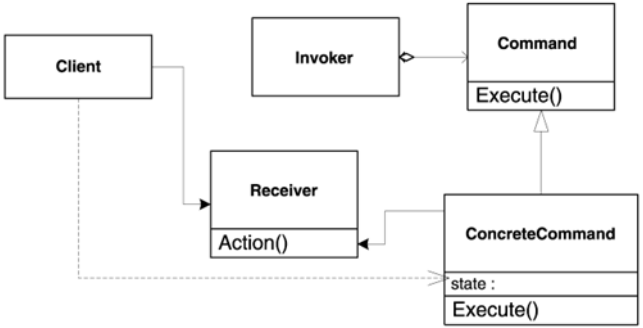
\includegraphics[width = 0.8\textwidth]{5.Functor/Functor1.png}
\end{figure}

\begin{enumerate}
\item The application (client) creates a \texttt{ConcreteCommand}
  object, passing it enough information to carry on a task. 
\item The application passes the \texttt{Command} interface of the
  \texttt{ConcreteCommand} object to the invoker. The invoker stores
  this interface.
\item  the invoker decides it's time to execute the action and fires
  \texttt{Command}'s Execute virtual member function. The virtual call
  mechanism dispatches the call to the \texttt{Concrete-Command }
  object, which takes care of the details. \texttt{ConcreteCommand}
  reaches the \texttt{Receiver} object (the one that is to do the job)
  and uses that object to perform the actual processing, such as
  calling its \texttt{Action } member function. Alternatively, the
  \texttt{ConcreteCommand} object might carry the processing all by
  itself. In this case, the receiver in Figure disappears.
\end{enumerate}

There are two important aspects of the Command pattern:
\begin{itemize}
\item \textbf{Interface separation}. The invoker is isolated from the
  receiver. 
\item \textbf{Time separation}. Command stores a ready-to-go
  processing request that's to be started later.
\end{itemize}

From an implementation standpoint, two kinds of concrete \texttt{Command}
classes can be identified:
\begin{enumerate}
\item All they do is call a member function for a \texttt{Receiver}
  object. We call them \textbf{forwarding commands}.
\item Others do tasks that are more complex. They might call member
functions of other objects, but they also embed logic that's beyond
simple forwarding. Let's call them active commands\textbf{}. 
\end{enumerate}
Because forwarding commands act much
like pointers to functions and their C++ colleagues, functors, we call
them \textbf{generalized functors}. 

\subsection{C++ Callable Entities}

A forwarding command is a callback on steroids, a generalized
callback. A callback is a pointer to a function that can be passed
around and called at any time.

In addition to simple callbacks, C++ defines many more entities that
support the function-call operator.  Let's enumerate all the things
that support \texttt{operator()} in C++:
\begin{itemize}
\item C-like functions
\item C-like pointers to functions
\item References to functions (which essentially act like const
  pointers to functions)
\item Functors, that is, objects that define an \texttt{operator()}
\item The result of applying \texttt{operator.*} or
  \texttt{operator->*} having a pointer to a member function
\end{itemize}
The objects that support \texttt{operator()} are known as
\textbf{callable entities}.

\subsection{\texttt{Functor} Class Template Skeleton}

in C++ a bald pointer to a polymorphic type does not strictly have first-class
semantics because of the ownership issue. To lift the burden of
lifetime management from \texttt{Functor}'s clients, it's best to provide
\texttt{Functor} with value semantics (well-defined copying and assignment).
\texttt{Functor} does have a polymorphic implementation, but that's hidden
inside it. We name the implementation base class \texttt{FunctorImpl}.

\begin{verbatim}
template <typename R, class TList>
class Functor{
public:
  Functor();
  Functor(const Functor&);
  Functor& operator=(const Functor&);
  explicit Functor(std::auto_ptr<Impl> spImpl);
private:
  // Handy type definition for the body type
  typedef FunctorImpl<R, TList> Impl;
  std::auto_ptr<Impl> spImpl_;
};
\end{verbatim}
The purpose of \texttt{Clone} is the creation of a polymorphic copy of
the \texttt{FunctorImpl} object.

\texttt{FunctorImpl} defines a polymorphic interface that abstracts a
function call.

\begin{verbatim}
template <typename R>
class FunctorImpl<R, NullType>{
public:
  virtual R operator()() = 0;
  virtual FunctorImpl* Clone() const = 0;
  virtual ~FunctorImpl() {}
};
template <typename R, typename P1>
class FunctorImpl<R, TYPELIST_1(P1)>{
public:
  virtual R operator()(P1) = 0;
  virtual FunctorImpl* Clone() const = 0;
  virtual ~FunctorImpl() {}
};
template <typename R, typename P1, typename P2>
class FunctorImpl<R, TYPELIST_2(P1, P2)>{
public:
  virtual R operator()(P1, P2) = 0;
  virtual FunctorImpl* Clone() const = 0;
  virtual ~FunctorImpl() {}
};
\end{verbatim}

Constructing from \texttt{auto\_ptr} is a clear statement to the
outside world that \texttt{Functor} takes ownership of 
the \texttt{FunctorImpl} object. Users of \texttt{Functor} will
actually have to type \texttt{auto\_ptr} whenever they invoke 
this constructor; we assume that if they type \texttt{auto\_ptr}, they
know what \texttt{auto\_ptr} is about.

\subsection{Implementing the Forwarding \texttt{Functor::operator()}}

\begin{verbatim}
template <typename R, class TList>
class Functor{
... as above ...
public:
  R operator()(){  return (*spImpl_)(); }
  R operator()(Parm1 p1){  return (*spImpl_)(p1); }
  R operator()(Parm1 p1, Parm2 p2){  return (*spImpl_)(p1, p2); }
};
\end{verbatim}

The  trick relies on the fact that \textbf{C++ does not instantiate member
  functions for templates until they are actually used}. If you try to call an overload
of \texttt{operator()} that doesn't make sense, the compiler tries to generate
the body of \texttt{operator()} and discovers the mismatch.

\subsection{Handling Functors}

\begin{verbatim}
template <class ParentFunctor, typename Fun>
class FunctorHandler: public FunctorImpl<
                       typename ParentFunctor::ResultType, 
                       typename ParentFunctor::ParmList>{
public:
  typedef typename ParentFunctor::ResultType ResultType;
  FunctorHandler(const Fun& fun) : fun_(fun) {}
  FunctorHandler* Clone() const{ 
    return new FunctorHandler(*this); 
  }
  ResultType operator()(){
    return fun_();
  }
  ResultType operator()(typename ParentFunctor::Parm1 p1){
    return fun_(p1);
  }
  ResultType operator()(typename ParentFunctor::Parm1 p1,typename ParentFunctor::Parm2 p2){
    return fun_(p1, p2);
  }
private:
  Fun fun_;
};
\end{verbatim}

The functor is stored by value, not by pointer. This is because, in general,
functors are meant to be this way—nonpolymorphic types with regular
copy semantics.

Given \texttt{FunctorHandler}'s declaration, it's easy to write the templated
constructor of \texttt{Functor} declared earlier in this section.

\begin{verbatim}
template <typename R, class TList>
template <typename Fun>
Functor<R, TList>::Functor(const Fun& fun) : spImpl_(new FunctorHandler<Functor, Fun>(fun)){}
\end{verbatim}

\textbf{\texttt{FuncotHandler} not only handles functor, function but
  also pointer and reference to functions.}

However, if the function is \textbf{overloaded}, the type of the function is no
longer defined.
\begin{verbatim}
void TestFunction(int i, double d){ cout << "TestFunction << endl; }
void TestFunction(int);
\end{verbatim}

There are two methods:
\begin{verbatim}
int main()
{
typedef void (*TpFun)(int, double);
// Method 1: use an initialization
TpFun pF = TestFunction;
Functor<void, TYPELIST_2(int, double)> cmd1(pF);
cmd1(4, 4.5);

// Method 2: use a cast
Functor<void, int, double> cmd2(static_cast<TpFun>(TestFunction));
cmd2(4, 4.5);
}
\end{verbatim}

\subsection{Argument and Return Type Conversions}

In an ideal world, we would like conversions to work for \texttt{Functor} just
as they work for regular function calls. 
\begin{verbatim}
const char* TestFunction(double, double){
  static const char buffer[] = "Hello, world!";
// It's safe to return a pointer to a static buffer
  return buffer;
}
int main(){
  Functor<string, TYPELIST_2(int, int)> cmd(TestFunction);
  // Should print "world!"
  cout << cmd(10, 10).substr(7);
}
\end{verbatim}

The function
\begin{verbatim}
string Functor<...>::operator()(int i, int j)
\end{verbatim}
forwards to the virtual function
\begin{verbatim}
string FunctorHandler<...>::operator()(int i, int j)
\end{verbatim}
whose implementation ultimately calls
\begin{verbatim}
return fun_(i, j);
\end{verbatim}
where \texttt{fun\_} has type \texttt{const char* (*)(double, double)}
and evaluates to \texttt{TestFunction}. When the compiler encounters
the call to \texttt{fun\_}, it compiles it normally. The compiler then
generates code to convert \texttt{i} and \texttt{j} to
\texttt{double}, and the result to \texttt{std::string}.

\subsection{Handling Pointers to Member Functions}

\begin{verbatim}
class Parrot{
public:
void Eat(){ cout << "Tsk, knick, tsk...\n"; }
void Speak(){ cout << "Oh Captain, my Captain!\n"; }
};
int main(){
  typedef void (Parrot::* TpMemFun)();
  TpMemFun pActivity = &Parrot::eat;
  
  Parrot geronimo;
  Parrot* pGeronimo = &geronimo;
  (geronimo.*pActivity)();
  (pGeronimo->*pActivity)();
  pActivity = &Parrot::Speak;
  (geronimo.*pActivity)();
}
\end{verbatim}

There is no C++ type for the result of \texttt{geronimo.*p-Activity}
and \texttt{pGeronimo->*pActivity}. Both are binary operations all
right, and they return something to which you can apply the 
function-call operator immediately, but that "something" does not have
a type. You cannot store the result of \texttt{operator.*} or
\texttt{operator->*} in any way.

Here's the implementation of \texttt{MemFunHandler}.
\begin{verbatim}
template <class ParentFunctor, typename PointerToObj, typename PointerToMemFn>
class MemFunHandler : public FunctorImpl<
                       typename ParentFunctor::ResultType,
                       typename ParentFunctor::ParmList>{
public:
  typedef typename ParentFunctor::ResultType ResultType;

  MemFunHandler(const PointerToObj& pObj, PointerToMemFn pMemFn) : pObj_(pObj), pMemFn_(pMemFn) {}
  MemFunHandler* Clone() const{ 
    return new MemFunHandler(*this); 
  }

  ResultType operator()(){
    return ((*pObj_).*pMemFn_)();
  }
  ResultType operator()(typename ParentFunctor::Parm1 p1){
    return ((*pObj_).*pMemFn_)(p1);
  }
ResultType operator()(typename ParentFunctor::Parm1 p1, typename ParentFunctor::Parm2 p2){
    return ((*pObj_).*pMemFn_)(p1, p2);
  }
private:
  PointerToObj pObj_;
  PointerToMemFn pMemFn_;
};
\end{verbatim}

Why is \texttt{MemFunHandler} parameterized with the type of the
pointer (\texttt{PointerToObj}) and not with the  type of the object
itself? i.e.
\begin{verbatim}
template <class ParentFunctor, typename Obj,
typename PointerToMemFn>
class MemFunHandler : public FunctorImpl<
                       typename ParentFunctor::ResultType,
                       typename ParentFunctor::ParmList>{
private:
  Obj* pObj_;
  PointerToMemFn pMemFn_;
public:
MemFunHandler(Obj* pObj, PointerToMemFn pMemFn) : pObj_(pObj), pMemFn_(pMemFn) {}
};
\end{verbatim}

The first implementation can store any type that acts as a pointer to an
object \textbf{but} the second is hardwired to store and use only
simple pointers, if you want to use smart pointers, there will be
wrong.

Moreover, the second version does not work for pointers to
\texttt{const}. Such is the negative effect of hardwiring type.

\begin{verbatim}
int main(){
  Parrot geronimo;
  Functor<> cmd1(&geronimo, &Parrot::Eat), cmd2(&geronimo, &Parrot::Speak);
  cmd1();
  cmd2();
}
\end{verbatim}

\subsection{Binding}

As soon as \texttt{Functor} is ready, new ideas come to mind. For
instance, we'd like to be able to convert from a type of
\texttt{Functor} to another. Think of a \texttt{Functor} as a
computation, and of its arguments as the \textbf{environment}
necessary to perform that computation,  binding allows
\texttt{Functor} to store part of the \textbf{environment} together
with the computation and to reduce progressively the environment
necessary at invocation time.

\begin{verbatim}
template <class Incoming>
class BinderFirst : public FunctorImpl<typename Incoming::ResultType, 
                     typename Incoming::Arguments::Tail>{
  typedef Functor<typename Incoming::ResultType,Incoming::Arguments::Tail> Outgoing;
  typedef typename Incoming::Parm1 Bound;
  typedef typename Incoming::ResultType ResultType;
public:
  BinderFirst(const Incoming& fun, Bound bound): fun_(fun), bound_(bound){}
  BinderFirst* Clone() const{ return new BinderFirst(*this); }
  ResultType operator()(){ return fun_(bound_); }
  ResultType operator()(typename Outgoing::Parm1 p1){
    return fun_(bound_, p1);
  }
  ResultType operator()(typename Outgoing::Parm1 p1,typename Outgoing::Parm2 p2){
    return fun_(bound_, p1, p2);
  }
private:
  Incoming fun_;
  Bound bound_;
};

template <class Fctor>
typename Private::BinderFirstTraits<Fctor>::BoundFunctorType
BindFirst(const Fctor& fun,typename Fctor::Parm1 bound){
  typedef typename private::BinderFirstTraits<Fctor>::BoundFunctorType Outgoing;
  return Outgoing(std::auto_ptr<typename Outgoing::Impl>(
                    new BinderFirst<Fctr>(fun, bound)));
}
\end{verbatim}


\subsection{Chaining Request}

\texttt{MacroCommand} class, a command that holds a
linear collection (such as a list or a vector) of
\texttt{Commands}. When a \texttt{MacroCommand} is executed, it
executes in sequence each of the commands that it holds.


\subsection{\texttt{Functor} Quick Facts}

\begin{itemize}
\item You can initialize a\texttt{ Functor} with a function, a
  functor, another Functor, or a pointer to an object and a pointer to
  a method.
\item You also can initialize \texttt{Functor} with a
  \texttt{std::auto\_ptr< FunctorImpl<R,TList> >}.
\item \texttt{Functor} supports automatic conversions for arguments
  and return values.
\item Manual disambiguation is needed in the presence of overloading.
\item \texttt{Functor} fully supports first-class semantics: copying,
  assigning to, and passing by value.
\item \texttt{Functor} is not polymorphic and is not intended to be
  derived from. If you want to extend \texttt{Functor}, derive from
  \texttt{FunctorImpl}.
\item  A call to \texttt{BindFirst} binds the first argument to a
  fixed value.
\item Multiple \texttt{Functors} can be chained in a single
  \texttt{Functor} object by using the \texttt{Chain} function. 
\item \texttt{FunctorImpl} uses the small-object allocator.
\end{itemize}

%%% Local Variables:
%%% mode: latex
%%% TeX-master: "../DesignPattern"
%%% End:


\newpage
\section{Singleton}

A singleton is an improved global variable. The improvement that
Singleton brings is that you cannot create a secondary object of the
singleton's type.

\subsection{Static Data + Static Functions != Singleton}

There is another pattern, the \textbf{Monostate pattern}:
\begin{verbatim}
class Font { ... };
class PrinterPort { ... };
class PrintJob { ... };

class MyOnlyPrinter{
public:
  static void AddPrintJob(PrintJob& newJob){
    if (printQueue_.empty() && printingPort_.available()){
      printingPort_.send(newJob.Data());
    }else{
      printQueue_.push(newJob);
    }
  }
private:
  // All data is static
  static std::queue<PrintJob> printQueue_;
  static PrinterPort printingPort_;
  static Font defaultFont_;
};
\end{verbatim}

The main problem is that static functions cannot be virtual, which
makes it difficult to change behavior without opening
\texttt{MyOnlyPrinter}'s code.

\subsection{The Basic C++ Idioms Supporting Singletons}

Most often, singletons are implemented in C++ by using some variation
of the following idiom:
\begin{verbatim}
class Singleton{
public:
  static Singleton* Instance(){
    if (!pInstance_)
      pInstance_ = new Singleton;
    return pInstance_;
  }
... operations ...
private:
  Singleton(); // Prevent clients from creating a new Singleton
  Singleton(const Singleton&); // Prevent clients from creating
  static Singleton* pInstance_; // The one and only instance
};
// Implementation file Singleton.cpp
Singleton* Singleton::pInstance_ = 0;
\end{verbatim}

If it's never used (no call to \texttt{Instance} occurs), the
\texttt{Singleton} object is not created. The advantage of the
build-on-first-request solution becomes significant if
\texttt{Singleton} is expensive to create and seldom used. 


An ill-fated temptation is to simplify things by replacing the pointer
\texttt{pInstance\_} in the previous example with a full Singleton
object.
\begin{verbatim}
class Singleton{
public:
  static Singleton* Instance() // Unique point of access{
    return &instance_;
  }
private:
  static Singleton instance_;
};
// Implementation file Singleton.cpp
Singleton Singleton::instance_;
\end{verbatim}

\texttt{instance\_} is initialized dynamically (by calling
\texttt{Singleton}'s constructor at runtime), whereas 
\texttt{pInstance\_} benefits from static initialization (it is a type
without a constructor initialized with a compile-time constant).

\begin{verbatim}
#include "Singleton.h"
int global = Singleton::Instance()->DoSomething();
\end{verbatim}

Depending on the order of initialization that the compiler chooses for
\texttt{instance\_} and \texttt{global}, the call to
\texttt{Singleton::Instance} may return an object that has not been
constructed yet.

\subsection{Enforcing the Singleton's Uniqueness}

 The default constructor and the copy constructor, the assignment
 operator are private.

 The problem with having Instance return a pointer is that callers
 might be tempted to \texttt{delete} it. To minimize the
chances of that happening, it's safer to return a reference:
\begin{verbatim}
// inside class Singleton
static Singleton& Instance();
\end{verbatim}

After the enumerated measures are added, Singleton's interface looks
like the following.
\begin{verbatim}
class Singleton{
public:
  Singleton& Instance();
  ... operations ...
private:
  Singleton();
  Singleton(const Singleton&);
  Singleton& operator=(const Singleton&);
  ~Singleton();
};
\end{verbatim}

\subsection{Destroying the Singleton}

If \texttt{Singleton} is not deleted, that's not a memory
leak. \textbf{Memory leaks appear when you allocate accumulating
dataand lose all references to it.  } 

However, \textbf{there is a leak, and a more insidious one: a resource
leak.}  Singleton's constructor may acquire an unbound set of
resources: network connections, handles to OS-wide mutexes and other
interprocess communication means and so on. The only correct way to
avoid resource leaks is to delete the Singleton object during the
application's shutdown.

The simplest solution for destroying the singleton is to \textbf{rely on
  language mechanisms}:
\begin{verbatim}
Singleton& Singleton::Instance(){
  static Singleton obj;
  return obj;
}
\end{verbatim}

This \texttt{Meyers singleton} relies on some compiler magic. When the
initializer is not a compile-time constant, or the static variable is
an object with a constructor,\textbf{ the variable is initialized at runtime
  during the first pass through its definition.}

In addition, the compiler generates code so that after initialization,
the pseudo-C++ representation of the generated code may look like the
following code:
\begin{verbatim}
Singleton& Singleton::Instance(){
  // Functions generated by the compiler
  extern void __ConstructSingleton(void* memory);
  extern void __DestroySingleton();
  // Variables generated by the compiler
  static bool __initialized = false;
  // Buffer that holds the singleton
  // (We assume it is properly aligned)
  static char __buffer[sizeof(Singleton)];
  if (!__initialized){
    // First call, construct object
    // Will invoke Singleton::Singleton
    // In the __buffer memory
    __ConstructSingleton(__buffer);
    // register destruction
    atexit(__DestroySingleton);
    __initialized = true;
  }
  return *reinterpret_cast<Singleton *>(__buffer);
}
\end{verbatim}

\textbf{The core is the call to the \texttt{atexit} function}, which
allows you to register functions to be automatically called during a
program's exit, in a last in, first out (LIFO) order. Each call to
atexit pushes its parameter on a private stack maintained by the C
runtime library.

\subsection{The Dead Reference Problem}

Assuming we implement \texttt{Keyboard}, \texttt{Display},
\texttt{Log} with three singletons as Meyers singletons. Assume that
after \texttt{Keyboard} is constructed successfully, \texttt{Display}
fails to initialize. \texttt{Display}'s constructor creates
\texttt{Log}, the error is logged.

At exit time,  \texttt{Log} is destroyed before \texttt{Keyboard}. If
for some reason \texttt{Keyboard} fails to shut down and tries to
report an error to \texttt{Log}, \texttt{Log::Instance} unwittingly
returns a reference to the "shell" of  a destroyed \texttt{Log}
object.  So \textbf{a reasonable singleton should at least perform
  dead-reference \emph{detection}.}

\begin{verbatim}
class Singleton{
public:
  Singleton& Instance(){
    if (!pInstance_){
      if (destroyed_){
        OnDeadReference();
      }else{
        Create();
      }
    }
    return *pInstance_;
  }
private:
  static void Create(){
    static Singleton theInstance;
    pInstance_ = &theInstance;
  }
  static void OnDeadReference(){
    throw std::runtime_error("Dead Reference Detected");
  }
  virtual ~Singleton(){
    pInstance_ = 0;
    destroyed_ = true;
  }

  Singleton *pInstance_;
  bool destroyed_;
  ... disabled 'tors/operator= ...
};

// Singleton.cpp
Singleton* Singleton::pInstance_ = 0;
bool Singleton::destroyed_ = false;
\end{verbatim}

\subsection{Addressing the Dead Reference Problem (I):
  The Phoenix Singleton}

The implementation of the Phoenix Singleton with a static variable is
simple. When we detect the dead reference, we create a new
\texttt{Singleton} object in the shell of the old one. (C++ guarantees
this is possible. Static objects' memory lasts for the duration of the
program.)

\begin{verbatim}
class Singleton{
  ... as before ...
  void KillPhoenixSingleton(); // Added
};
void Singleton::OnDeadReference(){
  Create();
  // Now pInstance_ points to the "ashes" of the singleton
  // - the raw memory that the singleton was seated in.
  // Create a new singleton at that address
  new(pInstance_) Singleton;
  // Queue this new object's destruction
  atexit(KillPhoenixSingleton);
  // Reset destroyed_ because we're back in business
  destroyed_ = false;
}
void Singleton::KillPhoenixSingleton(){
  pInstance_->~Singleton();
}
\end{verbatim}

The \texttt{new} operator that \texttt{OnDeadReference} uses is called
the placement \texttt{new} operator. The placement \texttt{new}
operator does not allocate memory; it only constructs a new object at
the address passed—in our case, \texttt{pInstance\_}.

\begin{verbatim}
#ifdef ATEXIT_FIXED
atexit(KillPhoenixSingleton);
#endif
\end{verbatim}

This measure has to do with an unfortunate omission in the C++
standard. The standard fails to describe what happens when you
register functions with atexit during a call made as the effect of
another \texttt{atexit} registration. To illustrate this problem,
let's write a short test program: 
\begin{verbatim}
#include <cstdlib>
void Bar(){ ... }
void Foo(){ std::atexit(Bar); }
int main(){
  std::atexit(Foo);
}
\end{verbatim}

They say that \texttt{Bar} will be called before \texttt{Foo} because
\texttt{Bar} was registered last, but at  the time it's registered,
it's too late for \texttt{Bar} to be first because \texttt{Foo} is
already being called.

\subsection{Addressing the Dead Reference Problem (II):
  Singletons with Longevity}

The Phoenix singleton breaks the normal lifetime cycle of a singleton,
which may confuse some clients.

Setting longevity control applies not only to singletons but also to
global objects in general. The concept emerging here is that of
longevity control and is independent of the concept of a singleton: 
\textbf{The greater longevity an object has, the later it will be
  destroyed. }

\begin{verbatim}
class SomeSingleton { ... };
class SomeClass { ... };
SomeClass* pGlobalObject(new SomeClass);
int main(){
  SetLongevity(&SomeSingleton().Instance(), 5);
  SetLongevity(pGlobalObject, 6);
}
\end{verbatim}
The function \texttt{SetLongevity} takes a reference to an object of
any type and an integral value (the longevity).

\textbf{You cannot apply SetLongevity to objects whose lifetimes are
  controlled by the compiler}, such as regular global objects, static
objects, and automatic objects. The compiler already generates code
for destroying them.

\begin{verbatim}
class SomeClass { ... };
int main(){
  SomeClass* pObj1 = new SomeClass;
  SetLongevity(pObj1, 5);
  static SomeClass obj2;
  SomeClass* pObj3 = new SomeClass;
  SetLongevity(pObj3, 6);
}
\end{verbatim}
A careful constraints analysis leads to the following design
decisions:
\begin{enumerate}
\item Each call to \texttt{SetLongevity} issues a call to
  \texttt{atexit}.
\item Destruction of objects with lesser longevity takes place before
  destruction of objects with greater longevity.
\item Destruction of objects with the same longevity follows the C++
  rule: last built, first destroyed. 
\end{enumerate}

In the example program, the rules lead to the following guaranteed
order of destruction: \texttt{*pObj1, obj2, *pObj3}.

\subsection{Implementing Singletons with Longevity}

\texttt{SetLongevity} maintains a hidden \texttt{priority queue},
separate from the inaccessible \texttt{atexit} stack. The core is the
priority queue data structure. We cannot use the standard
\texttt{std::priority\_queue} class because \textbf{it does not
  guarantee the ordering of the elements having the same priority.}

The elements that the data structure holds are pointers to the type
\texttt{LifetimeTracker}.
\begin{verbatim}
class LifetimeTracker{
public:
  LifetimeTracker(unsigned int x) : longevity_(x) {}
  virtual ~LifetimeTracker() = 0;
  friend inline bool Compare(unsigned int longevity, const LifetimeTracker* p){
  return p->longevity_ > longevity;
  }
private:
  unsigned int longevity_;
};
// Definition required
inline LifetimeTracker::~LifetimeTracker() {}

typedef LifetimeTracker** TrackerArray;
extern TrackerArray pTrackerArray;
extern unsigned int elements;
\end{verbatim}

There is only one instance of the \texttt{Tracker} type. Consequently,
\texttt{pTrackerArray} is exposed to all the Singleton problems just
discussed, \texttt{SetLongevity} must be available at any time. To
deal with this problem, \texttt{SetLongevity} carefully 
manipulates \texttt{pTrackerArray} with the low-level functions
\texttt{realloc}. if you call it with a zero size, it behaves like
\texttt{std::free}.

\begin{verbatim}
//Helper destroyer function
template <typename T>
struct Deleter{
  static void Delete(T* pObj){ delete pObj; }
};
// Concrete lifetime tracker for objects of type T
template <typename T, typename Destroyer>
class ConcreteLifetimeTracker : public LifetimeTracker{
public:
  ConcreteLifetimeTracker(T* p, unsigned int longevity, Destroyer d) : LifetimeTracker(longevity), pTracked_(p), destroyer_(d){}
  ~ConcreteLifetimeTracker(){ destroyer_(pTracked_); }
private:
  T* pTracked_;
  Destroyer destroyer_;
};

void AtExitFn(); // Declaration needed below

template <typename T, typename Destroyer>
void SetLongevity(T* pDynObject, unsigned int longevity,Destroyer d = Private::Deleter<T>::Delete){
  TrackerArray pNewArray = static_cast<TrackerArray>(
  std::realloc(pTrackerArray, sizeof(T) * (elements + 1)));
  if (!pNewArray) throw std::bad_alloc();
  pTrackerArray = pNewArray;
  LifetimeTracker* p = new ConcreteLifetimeTracker<T, Destroyer>(pDynObject, longevity, d);
  TrackerArray pos = std::upper_bound(pTrackerArray, pTrackerArray + elements, longevity, Compare);
  std::copy_backward(pos, pTrackerArray + elements,pTrackerArray + elements + 1);
  *pos = p;
  ++elements;
  std::atexit(AtExitFn);
}
\end{verbatim}

The \texttt{AtExitFn} function pops the object with the smallest
longevity and deletes it. Deleting the pointer to
\texttt{LifetimeTracker} invokes \texttt{ConcreteLifetimeTracker}'s
destructor, which in turn deletes the tracked object.
\begin{verbatim}
static void AtExitFn(){
  assert(elements > 0 && pTrackerArray != 0);
  LifetimeTracker* pTop = pTrackerArray[elements - 1];
  pTrackerArray = static_cast<TrackerArray>(std::realloc(pTrackerArray, sizeof(T) * --elements));
  delete pTop;
}
\end{verbatim}

\subsection{Putting It All Together}

\subsubsection{Decomposing \texttt{SingletonHolde} into Policies}

The three corresponding polices therefore are as follows:
\begin{itemize}
\item \textbf{Creation}. You can create a singleton in various ways.
\item \textbf{Lifetime}. We identified the following lifetime
  policies:
  \begin{enumerate}
  \item Following C++ rules—last created, first destroyed
  \item Recurring (Phoenix singleton)
  \item User controlled (singleton with longevity)
  \item Infinite (the "leaking" singleton, an object that's never destroyed)
  \end{enumerate}
\item \textbf{ThreadingModel}. Whether singleton is single threaded,
  is standard multithreaded or uses a nonportable threading model.
\end{itemize}

\subsubsection{Defining Requirements for \texttt{SingletonHolder}'s
  Policies}

The Creation policy must create and destroy objects, so it must expose
two corresponding functions. \texttt{Creator<T>} must
support the following calls:
\begin{verbatim}
T* pObj = Creator<T>::Create();
Creator<T>::Destroy(pObj);
\end{verbatim}

Lifetime decides the action to be taken if the application violates
the lifetime rules of the Singleton object. Hence:
\begin{itemize}
\item  If you need the singleton to be destroyed according to C++
  rules, then Lifetime uses a mechanism similar to \texttt{atexit}.
\item For the Phoenix singleton, Lifetime still uses an
  \texttt{atexit}-like mechanism but accepts the recreation of the
  Singleton object. 
\item For a singleton with longevity, Lifetime issues a call to
  \texttt{SetLongevity}.
\item For infinite lifetime, Lifetime does not take any action.
\end{itemize}

If \texttt{Lifetime<T>} is a class that implements the Lifetime
policy, the following expressions make sense:
\begin{verbatim}
void (*pDestructionFunction)();
Lifetime<T>::ScheduleDestruction(pDestructionFunction);
Lifetime<T>::OnDeadReference();
\end{verbatim}

\subsubsection{Assembling \texttt{SingletonHolder}}

\begin{verbatim}
template<class T,
  template <class> class CreationPolicy = CreateUsingNew,
  template <class> class LifetimePolicy = DefaultLifetime,
  template <class> class ThreadingModel = SingleThreaded>
class SingletonHolder{
public:
  static T& Instance();
private:
  static void DestroySingleton();
  SingletonHolder();

  typedef ThreadingModel<T>::VolatileType InstanceType;
  static InstanceType* pInstance_;
  static bool destroyed_;
};

template <...>
T& SingletonHolder<...>::Instance(){
  if (!pInstance_){
    typename ThreadingModel<T>::Lock guard;
    if (!pInstance_){
      if (destroyed_){
        LifetimePolicy<T>::OnDeadReference();
        destroyed_ = false;
      }
    pInstance_ = CreationPolicy<T>::Create();
    LifetimePolicy<T>::ScheduleCall(&DestroySingleton);
    }
  }
  return *pInstance_;
}

template <...>
void SingletonHolder<...>::DestroySingleton(){
  assert(!destroyed_);
  CreationPolicy<T>::Destroy(pInstance_);
  pInstance_ = 0;
  destroyed_ = true;
}
\end{verbatim}

%%% Local Variables:
%%% mode: latex
%%% TeX-master: "../DesignPattern"
%%% End:

\end{document}
%%% Local Variables:
%%% mode: xelatex
%%% TeX-master: t
%%% End:
